%
% IEEE Transactions on Microwave Theory and Techniques example
% Tibault Reveyrand - http://www.microwave.fr
%
% http://www.microwave.fr/LaTeX.html
% ---------------------------------------



% ================================================
% Please HIGHLIGHT the new inputs such like this :
% Text :
%  \hl{comment}
% Aligned Eq. 
% \begin{shaded}
% \end{shaded}
% ================================================



\documentclass[journal]{IEEEtran}

%\usepackage[retainorgcmds]{IEEEtrantools}
%\usepackage{bibentry}  
\usepackage{xcolor,soul,framed} %,caption

\colorlet{shadecolor}{yellow}
%\usepackage{color,soul}
\usepackage[pdftex]{graphicx}
\graphicspath{{../pdf/}{../jpeg/}}
\DeclareGraphicsExtensions{.pdf,.jpeg,.png}
\usepackage[cmex10]{amsmath}
%Mathabx do not work on ScribTex => Removed
%\usepackage{mathabx}
\usepackage{array}
\usepackage{mdwmath}
\usepackage{mdwtab}
\usepackage{eqparbox}
\usepackage{url}
\usepackage{lipsum}
\usepackage{booktabs}
\usepackage{rotating}
\usepackage{graphicx}
\usepackage{multicol}
\usepackage{multirow}
\usepackage{listings} % code blocks

\lstset{
  basicstyle={\small\ttfamily},
  breaklines=true,
  breakatwhitespace=true,
  tabsize=2
}

\renewcommand{\arraystretch}{1.3}
%\bstctlcite{IEEE:BSTcontrol}


%=== TITLE & AUTHORS ====================================================================
\begin{document}
\title{Fast Network Threat Detection based on the TRAbID dataset: An Analysis of Various Machine Learning Models }
\author{
Shrey Agarwal,
Ashwini Hiremath,
Ibrahim Khalid,
Harsh Shinde,
Justin Wang%
\thanks{Dr. Shih Yu Chang}
}
% The paper headers
\markboth{Fast Network Threat Detection}{Fast Network Threat Detection}


\maketitle



\begin{abstract}
In our increasingly digital world, network security is paramount. This project aims to enhance threat detection by training various machine learning models to classify network activities as either attacks or normal. Using the TRAbID dataset we trained models including Support Vector Machines, Logistic Regression, Naive Bayes, Random Forest, and XGBoost. These models were evaluated based on various metrics including F1 score and detection time. Results indicated that Gaussian Naive Bayes performed best in terms of F1 score, while Logistic Regression was the fastest. However, many models exhibited overfitting to the known dataset, not performing well with new attack data. This project looks at the challenges in deploying robust threat detection systems and highlights the potential of models like Naive Bayes for such tasks. Limitations included dataset size constraints and computational resources.% Future work should address these limitations to improve model generalization and efficacy in real-world scenarios.
\end{abstract}

\begin{IEEEkeywords}
Network anomaly detection, Machine Learning, Classification, Detection time
\end{IEEEkeywords}

\IEEEpeerreviewmaketitle



% === I. INTRODUCTION =============================================================
% =================================================================================
\section{Introduction}

\IEEEPARstart{I}{n} our ever increasing digital world, it is vital that we also have improved security over our networks. Based on the Cloudflare DDoS 2023 Q4 report \cite{cloudflare} and Verizon’s data breach report 2023 \cite{verizion}, there has been an increase in the number of cyber attacks, including network based attacks. By using live network data and classifying it as harmful or not, we can create a system that will improve the peace of mind of a user and allow them to use modern technology with confidence.

The primary objective of this project is to train various machine learning models for the classification of whether an activity on the network is a threat or not. The secondary objective of this project is to evaluate the machine learning models based on their performance, and computation time and cost in order to find the best model. This can be used to create a firewall application that uses the built machine learning model.

\section{Literature review}
Bagui et al. explored the UNSW-NB15 dataset using a hybrid approach that used k-means clustering followed by decision trees or Naive Bayes. Using decision trees, they were able to achieve a 99\% accuracy rate. \cite{bagui2019using} Bhati et al. used the KDDCUP99 dataset to explore the effectiveness of ensemble models such as AdaBoost and Random Forest. \cite{bhati2022ensemble} 

Zhou and Yang  developed an ``immune algorithm'' for detecting network anamolies using SVM. They were able to find that using such an algorithm, they were able to get an accuracy of 94\% with a detection time of 27 seconds for the entire test suite. \cite{zhou2006using}

Tavallaee et al. developed multiple machine learning models trained on the KDDCUP99 dataset, including Random Forest, Naive Bayes, and SVM. They were able to get accuracies of 92.8\%, 81.7\%, and 65.1\%, respectively. \cite{tavallaee2009detailed}

Viegas et al. generated the TRAbID dataset with the goal of providing a better dataset for training machine learning models. They used a novel approach of using various datasets with differing levels of similarity. They trained on this dataset using the Naive Bayes and Decision Tree algorithms. \cite{viegas2017toward}

Based on our short literature review among the listed papers and otherwise, there has not been a clear strive for creating a model with the goal of fast detection after training. We plan on furthering research in this regard by exploring the effectiveness of various machine learning techniques on the TRAbID dataset.

\section{Proposed methodology}
We are planning to use the TRAbID dataset \cite{viegas2017toward} as it provides a relevant dataset for the problem, this can be subject to change. The TRAbID dataset is sufficiently large, with 51 feature columns, including classification, made up of generated network traffic data. Our methodology will be to first explore this dataset using tools such as Pandas, MatPlotLib, and Sci-Kit Learn. This includes tasks such as identifying correlations, normalizing values, and selecting important features. Following this, we will work on training a few different types of models in order to determine which models perform the best at distinguishing network threats. Models we plan on training are: Support Vector Machines, Logistic Regression, Naive Bayes, Random Forest, and XGBoost. These selected models can be subject to change. We will compare the models based on accuracy, precision and recall, and speed of classification. The goal of this project is to find a model that, when deployed in a real life scenario, best performs analysis of raw network data and classifies it as `normal' or `attack' in terms of detection time and detection reliability.

% \subsection{Hypothesis}
% The anticipated results include improved organizational knowledge and awareness of the cyber threat landscape, allowing for improved readiness and response tactics. Furthermore, by adding to the body of knowledge on cybersecurity, these assessments hope to enhance defense systems and policies. The expected outcome of this research is to find a model that is able to quickly and accurately classify network traffic data. Future work based use cases on this research project would be to create a live network monitoring firewall application that can quickly run network traffic through a trained model and notify the user in case of a network based attack.

\section{Data Understanding and Exploration}
\label{data-understanding-and-exploation}
The dataset was downloaded from the original source as `arff' files. These files were quite large consisting of nearly 28,000,000 rows. Moreover, there was a huge imbalance in the dataset with nearly 99.7\% of the entries being `normal' entries. The exact numbers can be seen in Table \ref{table-class-distribution}.

\begin{table}[!htb]
    \centering
    \caption{Class distribution before and after reduction}
    \label{table-class-distribution}
    \begin{tabular}{llrrr}
         \toprule
Class&   \multicolumn{2}{c}{Before Reduction}& \multicolumn{2}{c}{After Reduction}\\
&  Normal& Attack& Normal&Attack\\
\midrule
Known & 28,618,341& 36,628& 48,432&36,628\\
Similar & 28,477,883& 10,440& 15,969&10,440\\
New & 28,391,902& 17,752& 58,138&17,752\\
\bottomrule
\end{tabular}
\end{table}

In order to reduce the computational complexity of this project as well as fix the class imbalance, we used a shell script to reduce the dataset. The results of this class re-balancing and data reduction can be seen in Table \ref{table-class-distribution}. The reduced files were saved as `csv' files locally for ease of use in data exploration and modelling. 


The first thing we need to understand about the data is how the known, similar, and new attacks are related to eachother and how they should be used to train and create the model. Based off the paper by Viegas et al. we can see their approach was based off Fig \ref{figure-known-similar-new}.\cite{viegas2017toward} To use the dataset as designed, we modelled our evaluation methods similar to theirs.

\begin{figure}[!htb]
    \centering
    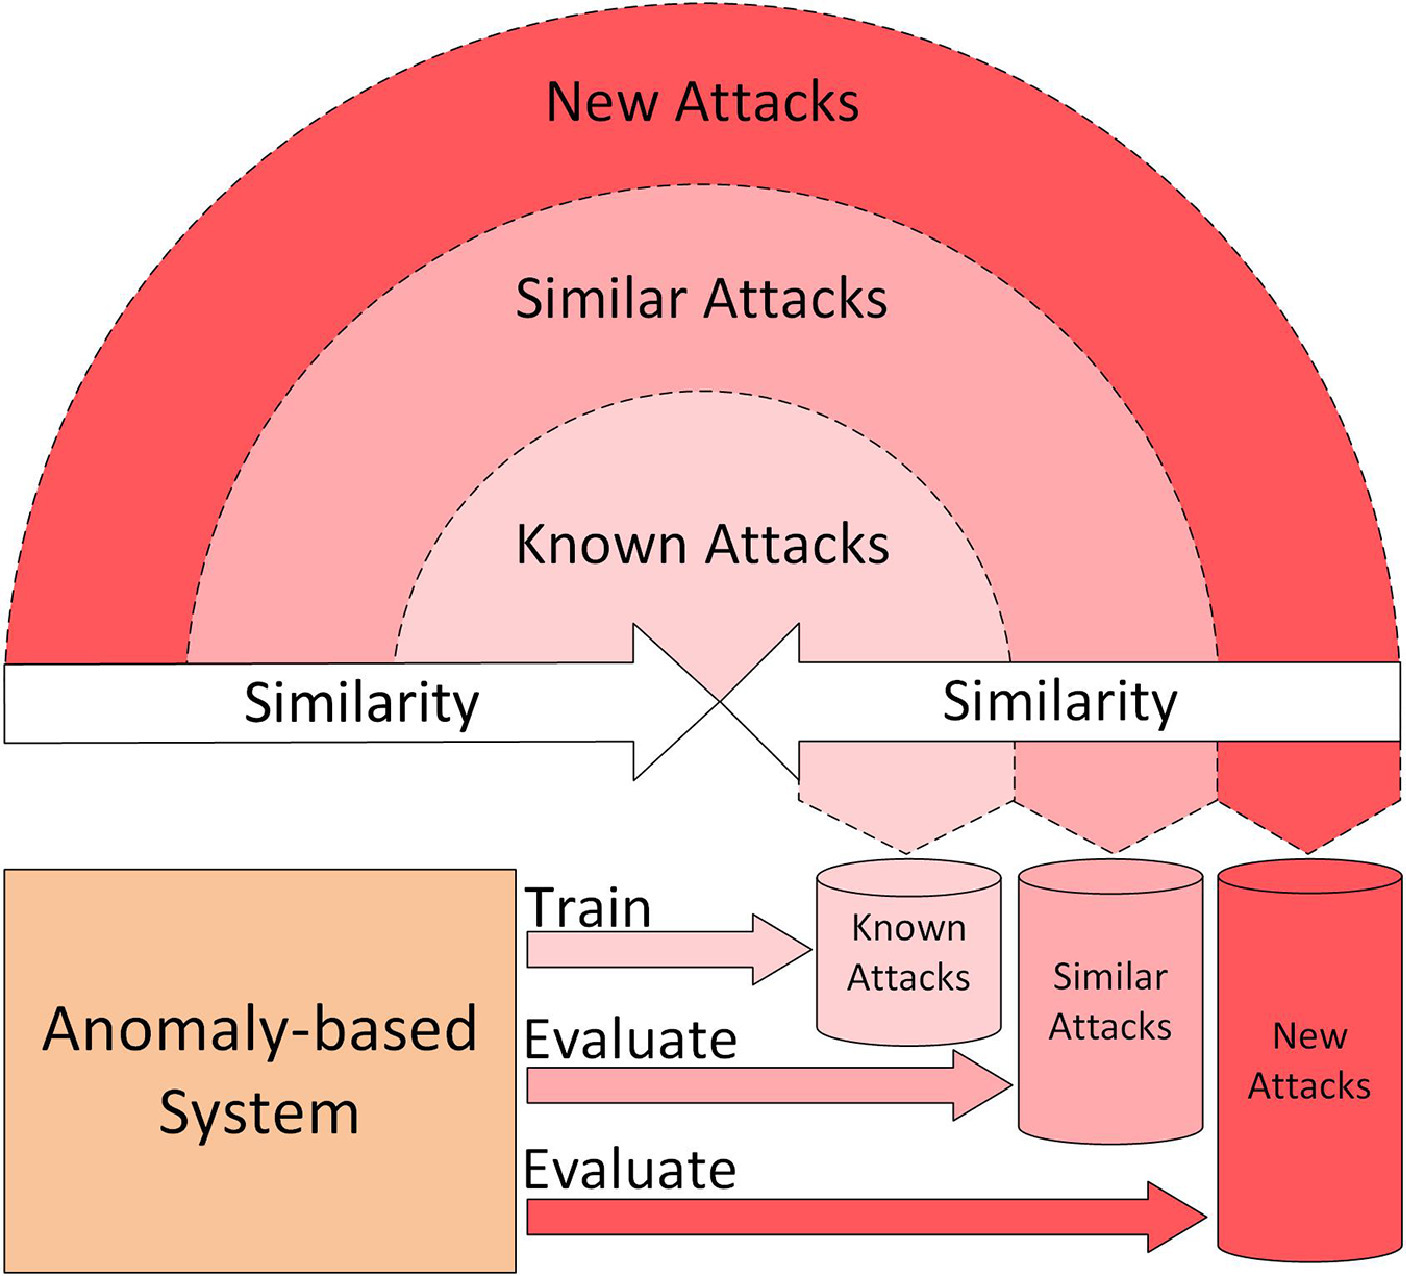
\includegraphics{figures/uploads/known_similar_new_attacks.jpg}
    \caption{Dataset relations and model evaluations}
    \label{figure-known-similar-new}
\end{figure}

Now that we know what dataset to use for what purpose, we began exploring the known dataset. There are 51 features in the dataset, all of which are listed in Table \ref{table-featurelist}

\begin{table}[!htb]
    \centering
    \caption{List of features}
    \label{table-featurelist}
    \begin{tabular}{>{\centering\arraybackslash}p{0.9\linewidth}}
    \toprule
 `ip\_type', `ip\_len', `ip\_id', `ip\_offset', `ip\_RF', `ip\_DF', `ip\_MF', `ip\_proto', `ip\_checksum', `udp\_sport', `udp\_dport', `udp\_len', `udp\_chk', `icmp\_type', `icmp\_code', `icmp\_chk', `tcp\_sport', `tcp\_dport', `tcp\_seq', `tcp\_ack', `tcp\_ffyn', `tcp\_fsyn', `tcp\_frst', `tcp\_fpush', `tcp\_fack', `tcp\_furg', `fr\_length', `conn\_status', `count\_fr\_dst\_src', `count\_serv\_src\_dst', `num\_bytes\_src\_dst', `num\_bytes\_dst\_src', `num\_bytes\_serv\_dst\_src', `num\_pushed\_dst\_src', `num\_syn\_fin\_src\_dst', `num\_fin\_src\_dst', `num\_fin\_dst\_src', `num\_ack\_dst\_src', `num\_syn\_src\_dst', `num\_rst\_src\_dst', `num\_rst\_dst\_src', `first\_packet', `first\_serv\_packet', `class'\\
 \bottomrule
    \end{tabular}
\end{table}




One of the first things we noticed was that the columns `ip\_RF', `ip\_DF' and `ip\_offset' were completely empty. These columns were removed as they should not affect our results greatly. Next, we performed a correlation analysis to see which of these remaining features were strongly correlated with the target feature. The results of this analysis can be seen in Table \ref{table-sorted-correlation}. The features with a greater than 0.1 absolute correlation are highlighted in bold.

\begin{table}[!htb]
    \centering
    \caption{Sorted correlation with target feature}
    \label{table-sorted-correlation}
    \resizebox{\linewidth}{!}{
    \begin{tabular}{lrlr}
\toprule
Feature & correlation&Feature & correlation\\\midrule
class&                    1.000000 & num\_syn\_dst\_src&         -0.017306\\
\textbf{tcp\_sport}&                0.376711 & count\_fr\_src\_dst&        -0.018505\\
\textbf{first\_serv\_packet}&        0.288401 & first\_packet&            -0.032560\\
\textbf{tcp\_fsyn}&                 0.183862 & num\_ack\_dst\_src&         -0.042007\\
\textbf{tcp\_ffyn}&                 0.179369 & num\_ack\_src\_dst&         -0.055285\\
\textbf{udp\_sport}&                0.159150 & count\_serv\_dst\_src&      -0.058866\\
\textbf{num\_rst\_dst\_src}&          0.148479 & icmp\_type&               -0.076590\\
tcp\_furg&                 0.081623 & tcp\_seq&                 -0.082221\\
ip\_id&                    0.070370 & tcp\_frst&                -0.089140\\
ip\_proto&                 0.068846 & ip\_type&                 -0.098455\\
tcp\_fpush&                0.068064 & \textbf{icmp\_chk}&                -0.106911\\
udp\_chk&                  0.050838 & \textbf{icmp\_code}&               -0.115398\\
udp\_dport&                0.043169 & \textbf{num\_bytes\_serv\_src\_dst}&  -0.205258\\
num\_syn\_fin\_dst\_src&      0.032562 & \textbf{conn\_status}&             -0.217683\\
num\_syn\_src\_dst&          0.023503 & \textbf{udp\_len}&                 -0.244732\\
num\_fin\_src\_dst&          0.018179 & \textbf{fr\_length}&               -0.249022\\
count\_fr\_dst\_src&         0.016557 & \textbf{ip\_len}&                  -0.265645\\
num\_syn\_fin\_src\_dst&      0.010139 & \textbf{num\_bytes\_src\_dst}&       -0.275082\\
num\_pushed\_src\_dst&      -0.005405 & \textbf{tcp\_dport}&               -0.302774\\
num\_pushed\_dst\_src&      -0.006834 & \textbf{ip\_DF}&                   -0.305169\\
num\_fin\_dst\_src&         -0.008403 & \textbf{tcp\_fack}&                -0.406649\\
num\_rst\_src\_dst&         -0.008925 & \textbf{tcp\_ack}&                 -0.456281\\
count\_serv\_src\_dst&      -0.010181 & \textbf{num\_bytes\_serv\_dst\_src}&  -0.520069\\
ip\_checksum&             -0.015762 & \textbf{num\_bytes\_dst\_src}&       -0.535816\\
\bottomrule
    \end{tabular}
    }
\end{table}



For further understanding, we performed principal component analysis (PCA) on all of the features as well as only those features with an absolute correlation greater than 0.1. PCA analysis is one of the common ways to reduce the dimensionality of a given dataset. In the case of machine learning, it means building a smaller model. The benefits of a smaller model are that they are more efficient and faster to train that models using the full dataset. One good benchmark for deciding the number of features to use from PCA reduction is to select the number of features that can help explain 95\% of the variance in the dataset. We found that when analyzing all the features present, we needed only 28 of the PCA transformed features to achieve 95\% cumulative explained variance. When analyzing only those features that had a greater than 0.1 absolute correlation, we needed only 10 of those PCA transformed features to achieve 95\% cumulative explained variance. See Fig. \ref{fig:pca-all} 

\begin{figure}[!htb]
    \centering
    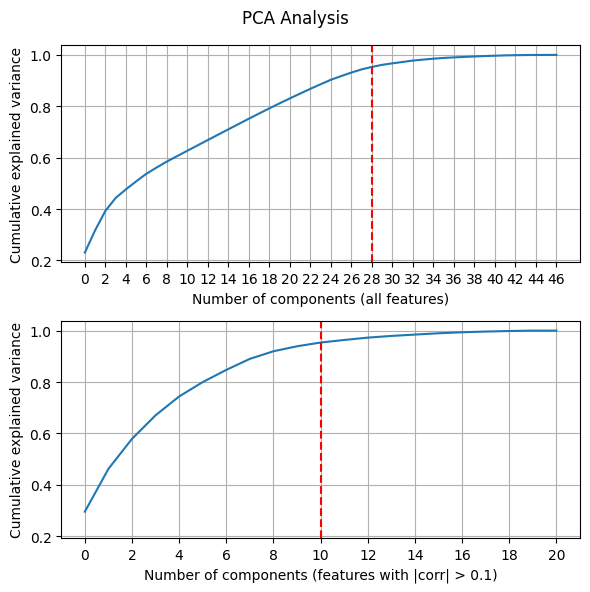
\includegraphics[width=1\linewidth]{figures//uploads/pca.png}
    \caption{PCA analysis on all features and features with correlation greater than 0.1. 95\% cumulative explained variance line highlighted}
    \label{fig:pca-all}
\end{figure}

Moreover, since that dataset itself covers various different ranges in different features, it was important that we also perform feature scaling. This was done through the use of the standard scaler class from the scikit learn library.

From our data understanding, it is clear that we can approach this problem via a number of different angles; we can use all the features, or a subset of highly correlated features, or we can use PCA reduced feature spaces, or some combination. 

The rest of this paper will look at how we used these different angles, or `pipelines', along with our selected models to find the answer to our problem. The pipeline that produces a dataset of all features scaled using the standard scaler will be called `\textit{scaled}'. The pipeline that produces a dataset of all those features which had an absolute correlation of 0.1 or more with the target feature and is scaled using the standard scaler will be called `\textit{corr, scaled}'. The pipeline that produces a dataset that explains 95\% of the variance in all features will be called `\textit{PCA}'. The pipeline that produces a dataset that explains 95\% of the variance of all those features which had an absolute correlation of 0.1 or more with the target feature will be called `\textit{corr, PCA}'.

Since our proposed methodology is trying to find the best model in terms of detection time and detection reliability, it is important to design our modelling to reflect that. While it is straight forward to test the models in terms of various metrics like accuracy and F1 score, it is harder to test their effectiveness in terms of time to detect. We need to develop our models and test suite in such a way that it allows us to do this with ease.

% For data undersstanding, we can prob have a quick paragraph describing the data

% Potentially stuff like the null values and so on
% correlation
% VIF
% PCA

% based on rubric, we also may need explanations about the relationships between the EDA results and our problem statement
% Rubric has a data preperation/preprocessing step; should we shoehorn it into this since our reasoning is also here, or should we make a new section?

\section{Modelling}

For modelling, we have selected 5 models to test against. These are: Naive Bayes, Support Vector Machines (SVM), Logistic Regression, Random Forest, and XGBoost. These models will be tested in all the pipelines mentioned in Section \ref{data-understanding-and-exploation}. Moreover, since we are testing the detection time of the models to correctly classify raw data, we need to design a benchmarking function that can cover all such scenarios. The pseudo code for this benchmark is as follows:
\begin{lstlisting}[numbers=left,numbersep=-2em,frame=lines]
    def benchmark(df, pipeline_fn, model):
        df_benchmark = pipeline_fn(df)
        X = df_benchmark[features]
        y = df_benchmark[target]
        y_pred = model.predict(X)
        save accuracy, precision, recall, F1
        start = time()
        for _ in ITER:
            df_benchmark = pipeline_fn(df)
            X = df_benchmark[features]
            model.predict(X)
        end = time()
        save (end - start / ITER)
\end{lstlisting}

Based on this code and the problem at hand, we developed the project architecture as described in Fig. \ref{fig:project-arch}. There we can see that all datasets are passed through the same selected pipeline function as defined in Section \ref{data-understanding-and-exploation}. The `Known' dataset is then split into a 70:15:15 ratio for training, validation, and testing, respectively. Using the training set of the known dataset, we train a baseline model. Then based on that, we perform hyper parameter tuning using the validation set. Once we have the best parameters for the given model, we train a new model on the training set using these parameters. This final model is not only tested on the testing set of the known data, but also on the `Similar' dataset and the `New' dataset. The scores of these tests are recorded and then the model performs the same test \lstinline{ITER} times. The benchmarking loop also performs data transformation on the raw data in order to test the transformation time as well. After all iterations are over, the average time per loop is recorded in milliseconds. For a good balance of reliable time measuring and computational resource availability, the \lstinline{ITER} loop was run a total of 10 times. This was repeated for all models and all pipelines.

\begin{figure*}
    \centering
    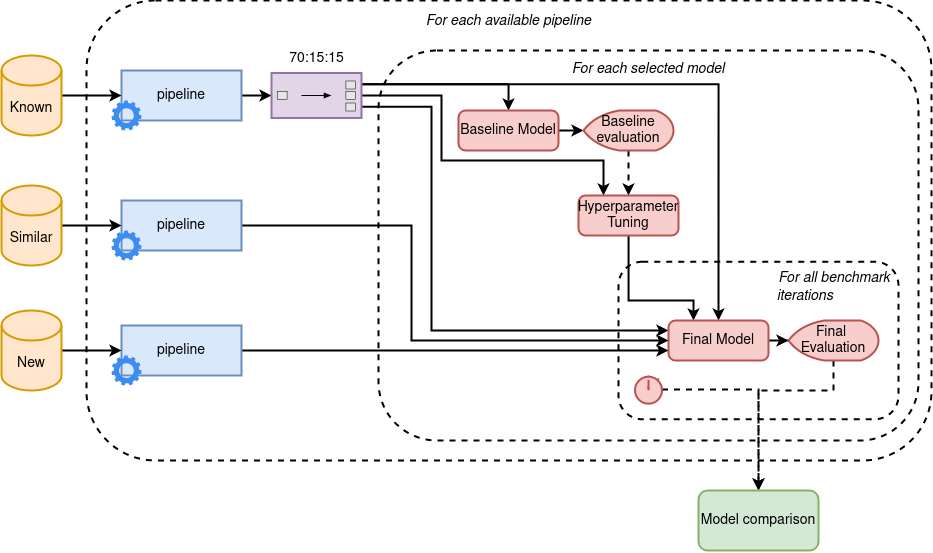
\includegraphics[width=\linewidth]{figures/uploads/project_arch.png}
    \caption{An overview flow diagram of the project as a whole}
    \label{fig:project-arch}
\end{figure*}

\subsection{Naive Bayes}
% Probably can include how naive bayes works, showing equations and what not
Naive Bayes is a supervised learning technique that is based on the Naive Bayes theorem. Unlike the other models in this report (SVM, Logistic Regression, and the tree based models), Naive Bayes is considered as a generative learning algorithm, focusing to model the distribution of inputs of a given class rather than learning which features are most important for discrimination. Some advantages of Naive Bayes include its simplicity and efficiency, the ability to handle high dimensional data, and its scalability. Some disadvantages include its assumption of conditional independence which causes to to be unrealistic, as well as its subjectability to the ``Zero Frequency'', which occurs when a feature does not exist in the training, causing the model to only predict zero.

For the modeling step, ComplementNB(), which is a version of MultinomialNB() that was designed to correct some its severe assumptions and works well with imbalanced data, as well as GaussianNB() was used. Additionally, hyperparameter tuning using GridSearchCV was utilized in order to improve results. ComplementNB() and GaussianNB() have different parameters, so they will be gone over in their respective sections.

\subsubsection{Complement Naive Bayes}
Complement Naive Bayes is a variation of Multinomial Naive Bayes that uses the complement of each class to calculate weights. As a result, this makes this model more suitable for imbalanced datasets, such as the TRAbID dataset. Complement Naive Bayes has the following parameters: alpha, force\_alpha, fit\_prior, class\_prior, and norm. Alpha is the smoothing parameter, force\_alpha will set alpha to 1e-10 if it is too low, fit\_prior is only used in edge cases with a single classes in the data, class\_prior is the prior probabilities of the classes but is not used in this implementation, and norm performs a second normalization of the weights. The parameter grid is as follows: 

\begin{lstlisting}
{
    "alpha": [0.001, 0.01, 0.1, 1, 10, 100, 1000],
    "force_alpha": [True, False],
    "fit_prior": [True, False],
    "norm": [True, False],
}
\end{lstlisting}

% The best performing params are all the same; featured in the table, but may have to explicity say bc the picture is small?
The best performing parameters for each test were the same for each model: 

\begin{lstlisting}
{
    "alpha": 0.001, 
    "fit_prior": True, 
    "force_alpha": True, 
    "norm": False
}
\end{lstlisting}
Featured in Fig. \ref{table-complement-results} are the results from the benchmark function using Complement Naive Bayes model after being going through hyperparameter tuning.

\begin{table}[!htb]
\caption{ComplementNB results}
\label{table-complement-results}
\centering
\resizebox{\linewidth}{!}{\begin{tabular}{llrrrrr}
\toprule
 &  & Accuracy & Precision & Recall & F1  \\
Pipeline & Dataset &  &  &  &  &  \\
\midrule
\multirow[c]{3}{*}{scaled} & Known & 0.940277 & 0.956870 & 0.903423 & 0.929379 \\
 & Similar & 0.972131 & 0.969336 & 0.959866 & 0.964578  \\
 & New & 0.794255 & 0.743730 & 0.183754 & 0.294697 \\
\cline{1-7}
\multirow[c]{3}{*}{corr, scaled} & Known & 0.944196 & 0.961817 & 0.907748 & 0.934001 \\
 & Similar & 0.977508 & 0.975010 & 0.967912 & 0.971448  \\
 & New & 0.796284 & 0.799373 & 0.172375 & 0.283596 \\

\cline{1-7}
\bottomrule
\end{tabular}
}
\end{table}

%\begin{figure*}[!htb]
%    \centering
%    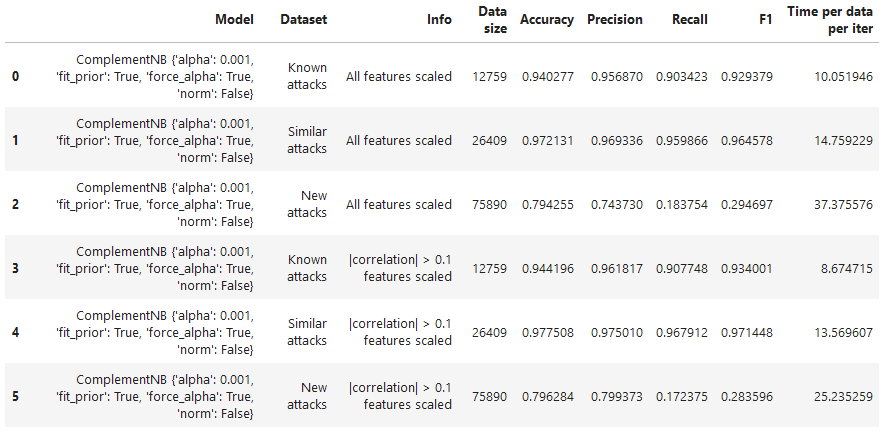
\includegraphics[width=\linewidth]{figures//naive_bayes/comp_nb_bench.png}
    % maybe we can use roc curves instead? they can fit in a single column...?
%    \caption{Complement Naive Bayes Benchmark}%ieee caption go on the bottom
%    \label{fig:comp_nb_bench}
%\end{figure*}

The results seem as expected, where the model performs well on known and similar attacks, while performing lackluster for new attacks. The best overall model for this test was on the scaled data, achieving an F1 score of 0.294697. This test, however, had some issues. The original preprocessing used for the benchmark function used a StandardScaler() and PCA. However, these methods gave negative values, which cannot be used by this model. As a result, the scaling method was changed to MinMaxScaler() and PCA was omitted. But by doing so, the process became different, making comparison a little more difficult, hence why Gaussian Naive Bayes was utilized to create tests that were more inline with the other models.

\subsubsection{Gaussian Naive Bayes}
Gaussian Naive Bayes generally performs better on continuous data, especially that which follows the normal distribution. While the data is not necessarily normal, it is continuous due to the StandardScaler() that is applied for the benchmark function. Unlike ComplementNB(), GaussianNB() is able to use negative values, allowing it to follow the same preprocessing and benchmark tests as the other models. This makes it much easier to make a comparison in terms of overall performance. GaussianNB() has two main parameters: priors, which are the prior probabilties for the classes, and var\_smoothing, which is the portion of the largest variance of all features that is added to variances for stability. In this case, priors was ignored and hyperparameter tuning was only performed based on var\_smoothing. The parameter grid used was \{'var\_smoothing': np.logspace(0,-9, num=100)\}, which creates 100 numbers between 1 and 1e-9. Featured in Table \ref{table-gaussiannb-results} are the results for Gaussian Naive Bayes.

\begin{table}[!htb]
\centering
\resizebox{\linewidth}{!}{\begin{tabular}{llrrrrr}
\toprule
 &  & Accuracy & Precision & Recall & F1 & Time (ms) \\
Pipeline & Dataset &  &  &  &  &  \\
\midrule
\multirow[c]{3}{*}{scaled} & Known & 0.817 & 0.707 & 0.991 & 0.825 & 9.917 \\
 & Similar & 0.795 & 0.661 & 0.987 & 0.792 & 19.195 \\
 & New & 0.691 & 0.313 & 0.268 & 0.289 & 50.295 \\
\cline{1-7}
\multirow[c]{3}{*}{corr, scaled} & Known & 0.826 & 0.716 & 0.995 & 0.833 & 4.697 \\
 & Similar & 0.806 & 0.672 & 0.994 & 0.802 & 7.989 \\
 & New & 0.700 & 0.319 & 0.251 & 0.281 & 28.354 \\
\cline{1-7}
\multirow[c]{3}{*}{PCA} & Known & 0.786 & 0.672 & 0.992 & 0.801 & 15.768 \\
 & Similar & 0.760 & 0.625 & 0.984 & 0.764 & 30.440 \\
 & New & 0.664 & 0.383 & 0.711 & 0.498 & 83.340 \\
\cline{1-7}
\multirow[c]{3}{*}{corr, PCA} & Known & 0.935 & 0.923 & 0.927 & 0.925 & 12.799 \\
 & Similar & 0.969 & 0.943 & 0.980 & 0.961 & 22.165 \\
 & New & 0.793 & 0.729 & 0.186 & 0.296 & 41.312 \\
\cline{1-7}
\bottomrule
\end{tabular}
}
\caption{GaussianNB results}
\label{table-gaussiannb-results}
\end{table}


This model still follows the trend of doing well on known and similar attacks while peforming mediocre on new attacks. However, this model seems to overfit less and performs significantly better on the new data. Based on what can be compared with ComplementNB(), the overall accuracies and computation time are quite comparable with each other. But, the precision to recall ratio is significantly different. For ComplementNB(), the precision is much greater than the recall, which implies that those models fail to differentiate the attack class well, but is normally correct when it does predict it. On the other hand, for GaussianNB(), the models were more balanced in terms of these metrics. The main difference stemmed from how the models performed on the new attacks.

The best performing test was using all of the features with 95\% PCA. This test used a var\_smoothing of 4.3287e-06. In terms of performance with known and similar attacks, it performed around the same, with F1 scores of 0.80096 and 0.76423 respectively. However, the new attacks drastically increased performance in terms of F1 score, achieving an F1 score of 0.49767, which is nearly double of those from the other tests. In terms of precision and recall, the precision of the model increased from around 0.3 to 0.38 while recall had massive increases, going from around 0.25 to 0.7. This means that this model is able to detect attacks better than the other models, but is prone to falsely flagging normal traffic. Despite having a slight accuracy drop, we believe that this is the best performing Naive Bayes model, mainly due to the class imbalance that exists in the data that skews accuracy. The precision of the model is approximately the same as the other tests, but the recall is significantly higher, going from around 0.25 to 0.7, implying that it is identifying threats and non threats much better than the others tests. For a problem like this, identifying problems, rather than being cautious, is imperative. Pictured in Fig. \ref{fig:gaus_roc} are the ROC curves for the known attacks, similar attacks, and new attacks for all of the tests using the GaussianNB() model. 

% use 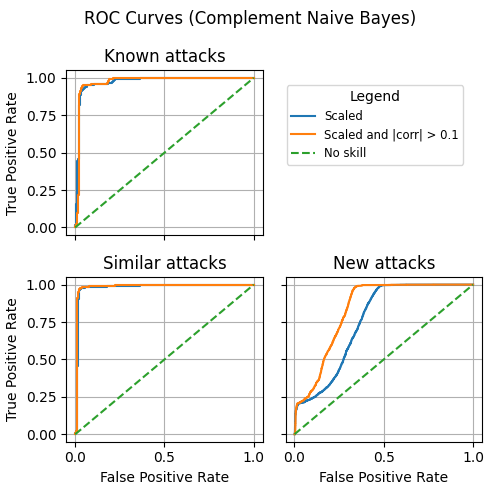
\includegraphics{figures/Complement Naive Bayes_roc_all_small.png}
\begin{figure}
    \centering
    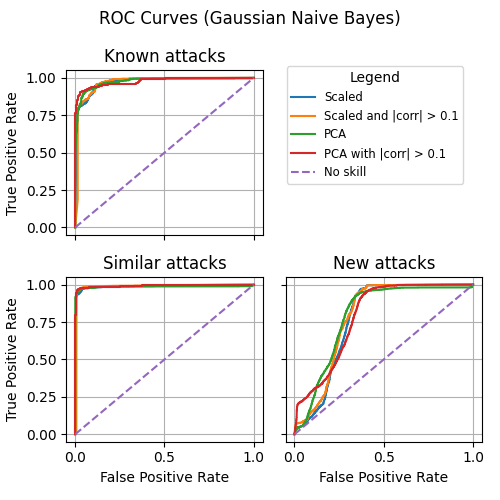
\includegraphics[width=\linewidth]{figures/Gaussian Naive Bayes_roc_all_small.png}
    \caption{Gaussian Naive Bayes ROC Curve}
    \label{fig:gaus_roc}
\end{figure}

An important thing to note is that the best performing model was using all features with 95\% PCA. The removal of features based on correlation was based on the known attacks data. This could imply that some of the features that were removed based on correlation may have been unimportant for known and similar, but were important for new attacks.




\subsection{Support Vector Machines}
Support Vector Machines (SVM) is a supervised machine learning method whose purpose is to separate two classes with an optimal hyperplane that maximizes the margin distances between the support vectors of each class and the hyperplane. This is a discriminative model, which means that it works by comparing the query point with the trained data points and bases the classification off of that. Some of the benefits of working with SVM include better performance on large feature spaces as well as it being memory efficient as it only requires the support vectors when making a classification. Some drawbacks of this model is that it is not easily interpretable and requires a lot of time to train. Theoretically, compared to the other models discussed in this paper, SVM should perform well. However, we will see later that out of all the models tested, SVM performed very poorly. One possible reason for this is that SVM has a tendency to over-fit to the dataset if there are too many samples. The results for SVM can be seen in Table \ref{table-svm-results}.

\begin{table}[!htb]
\centering
\resizebox{\linewidth}{!}{\begin{tabular}{llrrrrr}
\toprule
 &  & Accuracy & Precision & Recall & F1 & Time (ms) \\
Pipeline & Dataset &  &  &  &  &  \\
\midrule
\multirow[c]{3}{*}{scaled} & Known & 0.998 & 0.997 & 0.997 & 0.997 & 518.730 \\
 & Similar & 0.990 & 0.995 & 0.981 & 0.988 & 1037.263 \\
 & New & 0.767 & 0.656 & 0.009 & 0.019 & 2984.307 \\
\cline{1-7}
\multirow[c]{3}{*}{corr, scaled} & Known & 0.996 & 0.997 & 0.993 & 0.995 & 362.891 \\
 & Similar & 0.989 & 0.998 & 0.975 & 0.986 & 749.064 \\
 & New & 0.766 & 0.383 & 0.003 & 0.006 & 2147.515 \\
\cline{1-7}
\multirow[c]{3}{*}{PCA} & Known & 0.997 & 0.996 & 0.997 & 0.996 & 689.647 \\
 & Similar & 0.991 & 0.997 & 0.980 & 0.989 & 1514.054 \\
 & New & 0.767 & 0.620 & 0.008 & 0.016 & 3798.192 \\
\cline{1-7}
\multirow[c]{3}{*}{corr, PCA} & Known & 0.996 & 0.999 & 0.993 & 0.996 & 428.190 \\
 & Similar & 0.989 & 0.999 & 0.972 & 0.985 & 830.623 \\
 & New & 0.766 & 0.586 & 0.004 & 0.009 & 2294.048 \\
\cline{1-7}
\bottomrule
\end{tabular}
}
\caption{SVM results}
\label{table-svm-results}
\end{table}


We used SciKit-Learn's SVC classifier, which is based on the `LibSVM' implementation \cite{scikit-learn,chang2011libsvm}. Using this requires us to select some parameters for modelling. The main parameters we used for training are as follows.

The \lstinline{kernel} parameter controls which kernel the SVC classifier should use. The kernels supported by `LibSVM' are the linear kernel, polynomial kernel, RBF kernel, and sigmoid kernel. The benefit of using a specific kernel is how well the shape of the data fits to the given function. If there is a clear linear separation between the two classes, the best kernel will be the linear kernel, and so on.

There is a concept in SVM known as softmax margin. A softmax margin means that there can be some error in the margin's decision boundary, allowing for more flexible models. The \lstinline{C} parameter controls the strength of this regularization.

Finally, we have the \lstinline{gamma} parameter. This parameter takes on different meanings depending on the kernel being used. If the RBF kernel is used, then this parameter controls the radius of influence of training samples. If the polynomial kernel is used, this parameter controls the domination of higher degree terms. If the sigmoid kernel is used, this parameter controls the steepness of the sigmoid curve. This parameter is not used in the linear kernel. \cite{scikit-learn}

The parameter grid is therefore designed to test different combinations of each of these parameters in order to find the optimal model for the problem. The specific values for our parameter grid are shown as the following 
\begin{lstlisting}
{
    "C": [0.01, 0.1, 1, 10, 100, 1000],
    "kernel": ["poly", "rbf", "sigmoid", "linear"],
    "gamma": ["scale", "auto"],
}
\end{lstlisting}
Note, the `scale' value for \lstinline{gamma} means that the value will be set to $1/(n \times \sigma^{2}_{X})$, while setting it to `auto' will set the value to simply $1/n$. Where $n$ is the number of features and $\sigma^{2}_{X}$ is the variance of the input features. The optimal parameters for SVM based on given parameter grid can be seen in Table \ref{table-svm-params}.

\begin{table}[!htb]
\centering
\begin{tabular}{lllll}
\toprule
Pipeline & scaled & corr, scaled & PCA & corr, PCA \\
\midrule
C & 100 & 1000 & 100 & 1000 \\
gamma & scale & scale & auto & auto \\
kernel & rbf & rbf & rbf & rbf \\
\bottomrule
\end{tabular}
\caption{SVM best hyperparameters}
\label{table-svm-params}
\end{table}


\begin{figure}
    \centering
    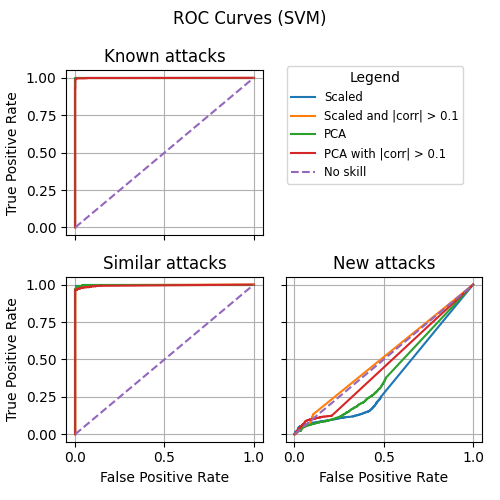
\includegraphics[width=\linewidth]{figures/SVM_roc_all_small.png}
    \caption{SVM ROC curves for all pipelines and each of the datasets tested. All models performed poorly except for the `corr, scaled' model, which just barely exceeds the no skill line}
    \label{fig:svm-roc}
\end{figure}

Given the results in Table \ref{table-svm-results}, we can see that even the best performing model only has a F1 score of 0.019 on the `New' dataset. One thing to note is that the best performing pipeline in SVM was the pipeline that had the most number of features, i.e. the `scaled' pipeline, which used all original features passed through a standard scaler. In terms of detection time, SVM performed the worst of all models and pipelines tested in this project. The ROC curves for this model's performance on all datasets and pipelines can be seen in Fig. \ref{fig:svm-roc}. 

Taking a close look at the ROC curves and the result table is that even the `testing' partition of the `Known' dataset has a nearly perfect prediction score across all pipelines, with the lowest F1 score being 0.995 and the lowest accuracy being 0.996. Similarly, with the `Similar' dataset, we can see that it too has very high scores. This might be indicative of the model overfitting to the `Known' dataset, and not being able to generalize to the concept of a harmful `attack' network event. 

\subsection{Logistic Regression}
Logistic regression is a statistical model used for classification problem. It is mainly used for predicting binary outcomes where the dependent variable is categorical. It is very easy to implement and interpret compared to other models. It saves computation costs and is efficient in scaling with large datasets. Moreover, it gives us probabilistic estimates which aid in efficient decision making but, it also has its drawbacks. It usually assumes a linear relationship between the features and target features. It is also sensitive to outliers and can affect model performance.
The results for Logistic Regression can be seen in Table \ref{table-logistic-regression-results}.
\begin{figure}
    \centering
    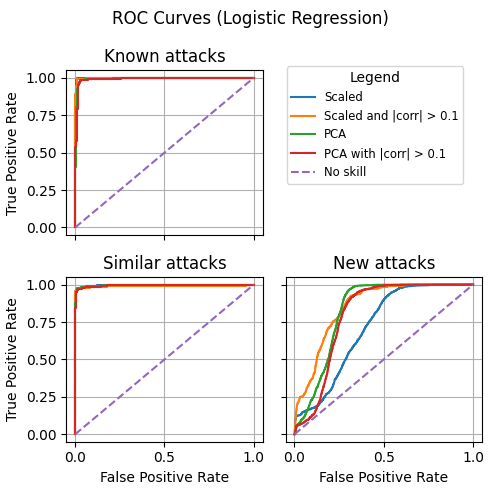
\includegraphics[width=\linewidth]{figures/Logistic Regression_roc_all_small.png}
    \caption{Logistic Regression ROC Curve}
    \label{fig:logreg_roc}
\end{figure}


\begin{table}[!htb]
\caption{Logistic Regression results}
\label{table-logistic-regression-results}
\centering
\resizebox{\linewidth}{!}{\begin{tabular}{llrrrrr}
\toprule
 &  & Accuracy & Precision & Recall & F1 & Time (ms) \\
Pipeline & Dataset &  &  &  &  &  \\
\midrule
\multirow[c]{3}{*}{scaled} & Known & 0.993 & 0.990 & 0.995 & 0.992 & 6.337 \\
 & Similar & 0.980 & 0.995 & 0.954 & 0.974 & 18.706 \\
 & New & 0.774 & 0.845 & 0.044 & 0.084 & 36.033 \\
\cline{1-7}
\multirow[c]{3}{*}{corr, scaled} & Known & 0.990 & 0.983 & 0.993 & 0.988 & 11.030 \\
 & Similar & 0.984 & 0.988 & 0.972 & 0.980 & 15.148 \\
 & New & 0.785 & 0.822 & 0.101 & 0.181 & 24.301 \\
\cline{1-7}
\multirow[c]{3}{*}{PCA} & Known & 0.980 & 0.974 & 0.979 & 0.977 & 16.595 \\
 & Similar & 0.983 & 0.983 & 0.972 & 0.978 & 22.989 \\
 & New & 0.767 & 0.533 & 0.042 & 0.078 & 72.396 \\
\cline{1-7}
\multirow[c]{3}{*}{corr, PCA} & Known & 0.978 & 0.974 & 0.977 & 0.975 & 7.628 \\
 & Similar & 0.982 & 0.981 & 0.973 & 0.977 & 13.880 \\
 & New & 0.767 & 0.546 & 0.033 & 0.061 & 30.205 \\
\cline{1-7}
\bottomrule
\end{tabular}
}
\end{table}



\subsection{Random Forest}
Table \ref{table-random-forest-results} shows the outcomes of using a Random Forest classifier to analyze several machine learning pipelines and quickly detect network threats on the TRAbID dataset. The performance measurements for each pipeline include accuracy, precision, recall, F1 score, and calculation time (measured in milliseconds). The dataset is divided into three categories: known, similar, and new threats. With a computation time of 140.314 ms, the Scaled pipeline achieves flawless scores across all measures, demonstrating excellent performance against known threats. With a computation time of 242.981 ms, it retains high accuracy (0.987), precision (1.000), recall (0.968), and F1 score (0.984) for similar threats. With an accuracy of 0.767, precision of 1.000, recall of 0.003, F1 score of 0.006, and the maximum computation time of 622.699 ms, New threats, on the other hand, show a marked decline in performance.

\begin{table}[!htb]
\caption{Random Forest results}
\label{table-random-forest-results}
\centering
\resizebox{\linewidth}{!}{\begin{tabular}{llrrrrr}
\toprule
 &  & Accuracy & Precision & Recall & F1 & Time (ms) \\
Pipeline & Dataset &  &  &  &  &  \\
\midrule
\multirow[c]{3}{*}{scaled} & Known & 1.000 & 1.000 & 1.000 & 1.000 & 140.314 \\
 & Similar & 0.987 & 1.000 & 0.968 & 0.984 & 242.981 \\
 & New & 0.767 & 1.000 & 0.003 & 0.006 & 622.699 \\
\cline{1-7}
\multirow[c]{3}{*}{corr, scaled} & Known & 1.000 & 1.000 & 1.000 & 1.000 & 68.079 \\
 & Similar & 0.989 & 1.000 & 0.971 & 0.985 & 111.215 \\
 & New & 0.767 & 0.923 & 0.005 & 0.011 & 308.599 \\
\cline{1-7}
\multirow[c]{3}{*}{PCA} & Known & 0.994 & 0.992 & 0.995 & 0.993 & 157.932 \\
 & Similar & 0.989 & 0.995 & 0.977 & 0.986 & 232.806 \\
 & New & 0.767 & 0.578 & 0.012 & 0.023 & 525.660 \\
\cline{1-7}
\multirow[c]{3}{*}{corr, PCA} & Known & 0.997 & 0.996 & 0.997 & 0.996 & 84.760 \\
 & Similar & 0.990 & 0.997 & 0.978 & 0.988 & 135.499 \\
 & New & 0.767 & 0.629 & 0.006 & 0.012 & 272.315 \\
\cline{1-7}
\bottomrule
\end{tabular}
}
\end{table}


With the shortest computation time of 68.079 ms, the Correlation and Scaled pipeline obtains flawless scores for known threats. With an accuracy of 0.989, precision of 1.000, recall of 0.971, F1 score of 0.985, and computation time of 111.215 ms, it outperforms the Scaled pipeline for Similar threats. It performs better than the Scaled pipeline when it comes to New threats, with a computation time of 308.599 ms, accuracy of 0.767, precision of 0.923, recall of 0.005, and F1 score of 0.011. With an accuracy of 0.994, precision of 0.992, recall of 0.995, F1 score of 0.993, and computation time of 157.932 ms, the PCA pipeline performs marginally worse for known threats. Performance drops much more for similar threats: 232.806 ms of computation time, 0.989 accuracy, 0.995 precision, 0.978 recall, and 0.986 F1 score. With an accuracy of 0.767, precision of 0.578, recall of 0.012, F1 score of 0.023, and computation time of 525.660 ms, the performance of the New threats is comparable to that of the Scaled pipeline.

With an accuracy of 0.997, precision of 0.996, recall of 0.997, F1 score of 0.996, and computation time of 84.760 ms, the Correlation and PCA pipeline performs well for known threats. With an accuracy of 0.990, precision of 0.997, recall of 0.978, F1 score of 0.988, and computation time of 135.499 ms, it performs well against similar threats. For New threats, performance is poor, with an accuracy of 0.767, precision of 0.629, recall of 0.006, F1 score of 0.012, and a computation time of 272.315 ms.

The ROC curves can be seen in \ref{fig:randomforest_roc}. ROC (Receiver Operating Characteristic) curves that indicate how well a Random Forest classifier performs in threat detection for three different scenarios: known assaults, similar attacks, and new attacks. Before the classifier is trained, various feature scaling and selection techniques are represented by each curve. The percentage of genuine positives that the model correctly detected is known as the True Positive Rate (TPR), sometimes referred to as sensitivity or recall. On the other hand, the percentage of actual negatives that the model mistakenly labeled as positives is known as the False Positive Rate (FPR). Plotting TPR against FPR at different threshold values, the ROC curve shows that higher performance is indicated by a closer distance to the top-left corner. ``PCA'' applies Principal Component Analysis to reduce dimensionality as discussed in section \ref{data-understanding-and-exploation}; ``PCA with $|corr|> 0.1$'' combines PCA with the correlation threshold; ``Scaled'' indicates standard scaling; ``Scaled and $|corr| > 0.1$'' retains only features with an absolute correlation greater than 0.1; and ``No skill'' represents a baseline model making random predictions. All techniques yield almost flawless identification for known attacks, demonstrating the effectiveness of the classifier when it has encountered similar patterns during training. Excellent performance is also demonstrated by similar attacks, indicating good generalization to variations of well-known methods. Performance varies for new attacks; the ``Scaled'' technique works best, suggesting that resilience against new threats depends on maintaining all characteristics with appropriate scaling. While approaches involving correlation thresholds perform less well and may exclude significant features, ``PCA'' performs quite well. These results emphasize the significance of thorough feature representation and suitable preprocessing, with scaling without further filtering offering the best generalization to novel threats and therefore improving threat detection systems' efficacy.

\begin{figure}
    \centering
    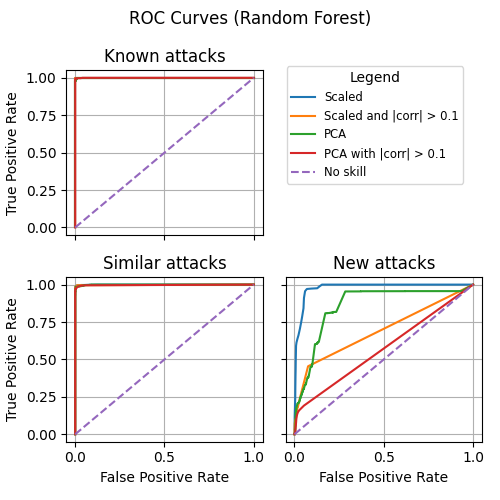
\includegraphics[width=\linewidth]{figures/Random Forest_roc_all_small.png}
    \caption{Random Forest ROC Curve}
    \label{fig:randomforest_roc}
\end{figure}

\subsection{XGBoost}
XGBoost is a popular supervised tree based algorithm that is popularly used in classification problems. This model is an example of an ensemble technique which follows the boosting principle. XGBoost is beneficial for several reasons. It tends to deliver a relatively high accuracy. It is also known for being very efficient when making predictions making them suitable for real time applications. XGBoost is not heavily impacted by outliers and is capable of handling both large and imbalanced datasets. The model is resistant to underfitting by default and has built-in parameters that can help to prevent overfitting. Along with the benefits, the model also has some drawbacks. One case is where despite having parameters that help it prevent overfitting, because of the model's nature, it can still be susceptible to it especially if not properly tuned. XGBoost's performance can also be a hit or miss on small or sparse datasets. This model can also take a while to train on large datasets since it is memory intensive. It can take up a good chunk of space within the RAM. Since this model has a lot of parameters in it, tuning the model can take time.  

In this case, we used the XGBClassifier available in the xgboost library to train this model. Generally speaking, this model should perform really well. In many other cases, it is generally considered the best performing model out of all. Here, the XGBoost model mostly performed as was expected for each test case. While this model was not the worst performing one, we can tell that it certainly did not perform the best. The results for XGBoost can be seen in Table \ref{table-xgbclassifier-results}.

\begin{table}[!htb]
\caption{XGBClassifier results}
\label{table-xgbclassifier-results}
\centering
\resizebox{\linewidth}{!}{\begin{tabular}{llrrrrr}
\toprule
 &  & Accuracy & Precision & Recall & F1 & Time (ms) \\
Pipeline & Dataset &  &  &  &  &  \\
\midrule
\multirow[c]{3}{*}{scaled} & Known & 1.000 & 1.000 & 1.000 & 1.000 & 39.135 \\
 & Similar & 0.989 & 0.999 & 0.973 & 0.986 & 51.636 \\
 & New & 0.762 & 0.276 & 0.010 & 0.019 & 126.805 \\
\cline{1-7}
\multirow[c]{3}{*}{corr, scaled} & Known & 1.000 & 1.000 & 1.000 & 1.000 & 22.749 \\
 & Similar & 0.991 & 0.999 & 0.978 & 0.988 & 46.507 \\
 & New & 0.780 & 0.751 & 0.089 & 0.159 & 122.587 \\
\cline{1-7}
\multirow[c]{3}{*}{PCA} & Known & 0.996 & 0.994 & 0.996 & 0.995 & 89.676 \\
 & Similar & 0.991 & 0.996 & 0.982 & 0.989 & 105.654 \\
 & New & 0.767 & 0.602 & 0.017 & 0.034 & 169.958 \\
\cline{1-7}
\multirow[c]{3}{*}{corr, PCA} & Known & 0.997 & 0.996 & 0.996 & 0.996 & 76.115 \\
 & Similar & 0.990 & 0.995 & 0.980 & 0.987 & 88.797 \\
 & New & 0.767 & 0.692 & 0.011 & 0.021 & 138.890 \\
\cline{1-7}
\bottomrule
\end{tabular}
}
\end{table}


Based on the result, we can see that the model performed the best on the `new' dataset through the correlation scaled pipeline. The best f1-score obtained was around 0.159. This result is better than some of the models, but still not as good in performance as others. This instance of the model on all versions training the `new' data also had the fastest training time at around 122 milliseconds.

To obtain the best possible results for every test case, we utilized hyperparameter tuning using GridSearchCV to train the model using the best possible parameter combination. The following parameter grid was utilized in to perform the hyperparameter tuning:

\begin{lstlisting}
{
    "max_depth": [10, 20, 30, 40, 50],
    "n_estimators": [100, 200, 400, 800],
    "learning_rate": [0.01, 0.1, 0.2],
    "gamma": [0.1, 0.5, 1],
    "scale_pos_weight": [0.1, 1, 5, 10]
}
\end{lstlisting}

The max\_depth parameter identifies the maximum depth of the tree. It controls the maximum number of nodes the exist in the tree from the root to the leaf node. This parameter is responsible for the complexity of the model. If the max\_depth value is set to being too high, there is the risk of overfitting. The higher the depth, the longer it will take for the model to train.

The n\_estimators focuses on the number of trees built or added to the model behind the scenes. Every subsequent tree learns from the previous trees mistakes. This higher the number of estimators, the more complex the model becomes. If the number of trees is too high, it can cause overfitting. The speed at which the model can train and predict the results also gets slower if the n\_estimators is too high. 

The learning\_rate is responsible for scaling the weights to determine the step size to take in each boosting round. It determines how quickly the model converges to its optimal point. Typically a lower learning rate will require more iterations for the model to reach convergence. The size of the learning\_rate can impact the accuracy of the model. Typically if there are a high number of n\_estimators, then a lower learning rate yields to a model generalizing better and yielding to more accurate results while also reducing the risk of overfitting. 

The gamma parameter represents the minimum loss reduction needed for a split to occur at a leaf node. Typically the higher the gamma value, the more the tree pruning there is. This prevents any unnecessary splits from, occurring. Increasing gamma also reduces the model complexity which can help reduce the risks of overfitting. Gamma acts as the regularization parameter in XGBoost which works to prevent overfitting from occurring. 

The scale\_pos\_weight addresses the balance between positive and negative classes. In other words, it handles class imbalance issues in a dataset with binary classification. Using this parameter can help to increase the accuracy or f1-score and try to prevent super skewed results from being obtained if the data is imbalanced. 

Figure \ref{fig:xgboost_roc} provides the ROC curves showing the distribution of classification for all datasets.
\begin{figure}
    \centering
    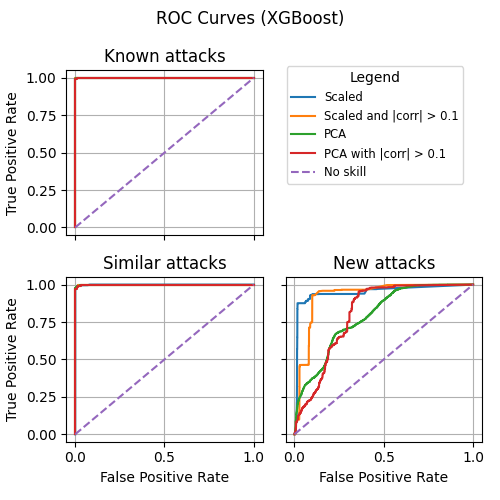
\includegraphics[width=\linewidth]{figures/XGBoost_roc_all_small.png}
    \caption{ROC curves for XGBoost}
    \label{fig:xgboost_roc}
\end{figure}

Based on the curves for `new attacks', we can tell the model performed as expected. All the cases involving PCA performed worse than any of the scaled versions. The red curve representing the PCA with correlation pipeline shows more variance in results compared with the other cases. For every other dataset in each pipeline, the f1-score is never below 0.9. For every instance of the `new' dataset, the result, again, appears to be the best in the pipeline involving scaled with correlation and also has the fastest computation time. For every other pipeline, the f1-score is below 0.05. XGBoost's overall performance was generally reasonable, but not as good as how Naive Bayes or Logistic Regression performed. 

\section{Evaluating Results and comparing}

Now that we have all the various models trained, we can run all models on the same system to perform a comparative benchmark. Since false positives and false negatives are both bad for our application, we will primarily compare the models using F1 score. At the same time, we also need to find the best model in terms of detection time. We will compare the models in these regards using the `New' dataset as this is most important dataset for making sure that the selected model performs well in the real world.

The tables comparing best models in terms of F1 score can be seen in Table \ref{table-top-5-f1-new}. The best performing model in terms of F1 score was Gaussian Naive Bayes using all features with 95\% PCA.

\begin{table}[!htb]
\caption{Top 5 models by F1 on New data}
\label{table-top-5-f1-new}
\centering
\begin{tabular}{rllr}
\toprule
Rank & Model & Pipeline & F1 \\
\midrule
1 & GaussianNB & PCA & 0.498 \\
2 & GaussianNB & corr, PCA & 0.296 \\
3 & GaussianNB & scaled & 0.289 \\
4 & GaussianNB & corr, scaled & 0.281 \\
5 & Logistic Regression & corr, scaled & 0.181 \\
\bottomrule
\end{tabular}
\end{table}


The tables comparing best models in terms of detection time can be seen in Table \ref{table-top-5-time-(ms)-new}. The best performing model in terms of speed was Logistic Regression using scaled features that had a correlation of greater than 0.1.

\begin{table}[!htb]
\caption{Top 5 models by Time (ms) on New data}
\label{table-top-5-time-(ms)-new}
\centering
\begin{tabular}{rllr}
\toprule
Rank & Model & Pipeline & Time (ms) \\
\midrule
1 & Logistic Regression & corr, scaled & 24.301 \\
2 & GaussianNB & corr, scaled & 28.354 \\
3 & Logistic Regression & corr, PCA & 30.205 \\
4 & Logistic Regression & scaled & 36.033 \\
5 & GaussianNB & corr, PCA & 41.312 \\
\bottomrule
\end{tabular}
\end{table}


By looking at both of these tables, it is clear that both Logistic Regression and Gaussian Naive Bayes perform the best of all the models in this project. Gaussian Naive Bayes far exceeds all models in terms of F1 score, even when using any of the available pipelines. Logistic regression and Gaussian Naive Bayes are both equally represented in the top 5 in terms of detection time with all models approximately around 30ms.

% In terms of both tables, Naive Bayes and Logistic Regression outperformed every other model. This could be due to their probabilistic nature.

\section{Deployment}
% We have two potential deployment strategies in mind. First, an online hosted application using platforms such as Streamlit could be created for research purposes. Second, for a more real-world use-case, applications such as Wireshark could be used to obtain live network traffic data, allowing us to create a firewall application that runs on the user's system with the selected best model.

We have two potential deployment strategies for this project. First, we could make this project available online for research purposes. Second, we could select the `best' model from this project and make it available as an end user firewall application.

For the first possible deployment solution, we can host all model pickle files to platforms such as HuggingFace. The use case for this deployment solution is that it will allow other researchers and developers to use our models when performing studies. These online platforms will allow easy scaling to a vast number of users across the world as long as the compute is available. One drawback to this approach is that there would be a continuous cost to the account owners.

For the second approach, we can create a user application in Python that is installed to the user's network. This application will come bundled with the best model from this study, Gaussian Naive Bayes, and will apply the best pipeline to live network traffic. This live network traffic will be evaluated by the model and will alert the user in case of detection of malicious network activity. Scaling this will be relatively simple as each user will need to download and install the application, only providing their own computation resources.

For either of these deployment strategies, we would first need to improve the models and provide the model saved to disk. This can be done with the \lstinline{pickle} package in Python.

% Jots for the "discussion" part
% Our model needs to be updated every now and then
% Model has to be fast enough to handle a stream of real time data
% idk could use a platform like kafka or something...
% some bs about parallelization to allow for faster computations idk


\section{Conclusion}

% the overfitting thing; transitions into how naive bayes had the best overall f1; generative v discriminative as a potential answer?
Based on our poor results, we believe that the majority of models are massively overfitting. For almost every model, every statistic for the known and similar datasets are 1, or very close to it, while the F1 scores for new attacks are extremely low. This is likely due to the fact that the new attacks data is very dissimilar with the known and similar attacks. As a result, the models are unable to properly predict new attacks. The only model that seemed to combat this was Naive Bayes. This could be because Naive Bayes is considered a generative model whereas the other models are considered discriminative. Discriminative models identifies decision boundaries and categorizes based on that. On the other hand, generative models learns the probability distribution of the data.

This project had a few limitations and things that could be improved on. The original known attacks data had over 28 million rows while we only used 100,000. This was due to a lack of sufficient hardware and computation power. Additionally, given that every model was unable to perform well, we were unable to significantly link the known and similar attacks to the new attacks.

\ifCLASSOPTIONcaptionsoff
  \newpage
\fi

\bibliographystyle{IEEEtran}
\bibliography{IEEEabrv,Bibliography}

% \begin{IEEEbiography}[{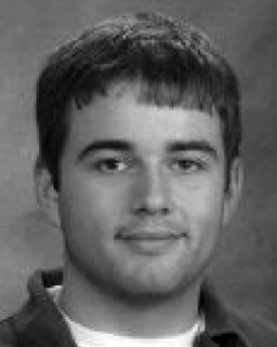
\includegraphics[width=1in,height=1.25in,clip,keepaspectratio]{photo/mike.png}}]{Michael Roberg}
% Do we need a bio section? We should ask the professor
% \end{IEEEbiography}
\vfill
\end{document}